\documentclass[9pt,xcolor=table,hyperref=unicode]{beamer}
\usetheme{Berkeley}
\usepackage[utf8]{vietnam}
\usepackage{tikz}
\usepackage{hyperref}
\usepackage{booktabs, multicol, multirow}
\usepackage{adjustbox}
\usepackage{array}
\usepackage{tikz}
\usetikzlibrary{positioning}
\newcolumntype{x}[1]{>{\centering\arraybackslash\hspace{0pt}}p{#1}}
\graphicspath{ {images/} }
\usepackage{xcolor}

\setbeamerfont{page number in head/foot}{size=\small}
\setbeamertemplate{footline}[frame number]

\newcommand{\inlineitem}{%
\leavevmode\usebeamertemplate{itemize item}
}
\newcounter{newenumi}
\setcounter{newenumi}{1}

\newcommand{\inlineenum}{%
 {%
 \setcounter{enumi}{\thenewenumi}%
 \leavevmode\usebeamertemplate{enumerate  item}
 \stepcounter{newenumi}
 \setcounter{enumi}{0}
 }
}

\newcommand{\resetinlineenum}{
 \setcounter{newenumi}{1}
}

\setbeamertemplate{footline}{% 
  \hfill% 
  \usebeamercolor[fg]{page number in head/foot}% 
  \usebeamerfont{page number in head/foot}% 
  \insertframenumber%  
  \kern1em\vskip2pt% 
}

\setbeamercolor{page number in head/foot}{fg=black}

%---------------SET FOR DIAGRAM------------------------------
\usetikzlibrary{arrows,chains,positioning,scopes}

\tikzset{
    block/.style={draw,thick,text width=5em,minimum height=6.5em,minimum width=5em,align=center},
    arrow/.style={->, thick}
}

\begin{document}
	\setbeamertemplate{sidebar left}[sidebar theme]
	\setbeamertemplate{enumerate/enumerate body begin}{\HUGE}
	
	\title{Luận văn tốt nghiệp}
	\subtitle{\fontsize{16pt}{16}\selectfont Phân giải đồng tham chiếu cho \\ các đối tượng và thuộc tính trong \\ khai khoáng ý kiến}
	\author[]{
		\normalsize
		\begin{tabular}{ll}
			Nguyễn Trọng Nghĩa & 51202370 \\
			Nguyễn Đăng Trang & 51203957 \\
			 & 
		\end{tabular}
		\break
		\begin{tabular}{ll}
			GVHD & GS.TS Phan Thị Tươi \\
			GVPB & GS.TS Cao Hoàng Trụ
		\end{tabular}
	}
	\institute{Đại học Bách Khoa TP. Hồ Chí Minh}
	\date{\today}
	
	\begin{frame}
		\Large
		\maketitle
	\end{frame}

	\begin{frame}{Nội dung trình bày}
		\LARGE
		\begin{enumerate}
			\itemsep1.5em 
			\item{Tổng quan đề tài}
			\item{Các công trình liên quan}
			\item{Phương pháp đề xuất}
			\item{Thực nghiệm và đánh giá}
			\item{Tổng kết}
		\end{enumerate}
	\end{frame}


	\section{Tổng quan đề tài}
	\begin{frame}
		\frametitle{Tổng quan đề tài}
		\begin{block}{Giới thiệu đề tài}
			\begin{itemize}
				\item{\textit{Phân giải đồng tham chiếu} hướng đến việc tìm kiếm những từ, cụm từ hoặc ngữ cùng chỉ đến một khái niệm, thực thể trong thế giới thực.}
				\item{Nội dung đề tài: \textit{Phân giải đồng tham chiếu} cho \textit{đối tượng} và \textit{thuộc tính} trong các \textit{văn bản chứa ý kiến}.}				
			\end{itemize}
		\end{block}		
		\begin{block}{Ví dụ}			
			\textit{Beckham} will visit Vietnam tomorrow. \textit{He} will attend a football event in Saigon.
		\end{block}			
	\end{frame}
	
	\begin{frame}
		\frametitle{Tổng quan đề tài (tt)}
		\begin{block}{Động cơ thực hiện đề tài}
			\begin{itemize}	
				\item{Thương mại điện tử đang phát triển mạnh mẽ và người dùng ngày càng có nhu cầu thể hiện ý kiến lên các sản phẩm trên mạng.}
				\item{Nếu không có phân giải đồng tham chiếu cho các đối tượng và thuộc tính, ý kiến của người viết rất có thể sẽ được gán không đúng cho các thực thể.}								
			\end{itemize}		
		\end{block}		
		\begin{block}{Ví dụ}						
			\textit{The Galaxy III} is pretty cool. \underline{It}'s a plastic phone, but \underline{it} feels solid even though \underline{it}'s very light. \textit{The screen} looks great. \underline{It} is very sharp.
		\end{block}
	\end{frame}

	\begin{frame}
		\frametitle{Tổng quan đề tài (tt)}
		\begin{block}{Mục tiêu đề tài}
			Tìm ra các từ/cụm từ trong văn bản chứa ý kiến cùng chỉ về một đối tượng hoặc thuộc tính nào đó, tức là tìm các chuỗi đồng tham chiếu của đối tượng và thuộc tính.
		\end{block}		
		\begin{block}{Phạm vi đề tài}
			\begin{itemize}
				\item{Giả định rằng các đối tượng và thuộc tính đã được tìm ra \footnotemark \textsuperscript{,} \footnotemark}
			\end{itemize}
			\footnotetext[1]{Minqing Hu and Bing Liu. 2004.
				\textit{Mining and Summarizing Customer Reviews}.
				In Proceedings of the ACM SIGKDD International Conference on Knowledge Discovery and Data Mining (KDD-2004), Aug 22-25, 2004, Seattle, Washington, USA.
			}
			\footnotetext[2]{A-M. Popescu and O. Etzioni. 2005. 
				\textit{Extracting product features and opinions from reviews}.
				EMNLP’05.
			}
		\end{block}
	\end{frame}


	\section{Các công trình liên quan}
	\begin{frame}
		\frametitle{Các công trình liên quan}
		\begin{block}{Đồng tham chiếu}
			Kể từ những năm 1960 đến nay đã có nhiều công trình nghiên cứu.
			\begin{itemize}
				\item{Các mô hình: Mô hình cặp, mô hình hướng thực thể, mô hình xếp hạng}
				\item{Các hướng tiếp cận: Học có giám sát, học không giám sát, hệ thống luật}
			\end{itemize}
		\end{block}
		\begin{block}{Đồng tham chiếu trong khai khoáng ý kiến}
			\begin{itemize}
				\item{Stoyanov và Cardie (2006): Phân giải đồng tham chiếu cho chủ thể ý kiến \footnotemark}
				\item{Ding và Liu (2010): Phân giải đồng tham chiếu đối tượng và thuộc tính \footnotemark}
			\end{itemize}
		\end{block}
		\footnotetext[3]{Veselin Stoyanov and Claire Cardie. 2006.
			\textit{Partially supervised coreference resolution for opinion summarization through structured rule learning}.
			In Proceedings of the 2006 Conference on Empirical Methods in Natural Language
			Processing (EMNLP), pages 336-344.}
		\footnotetext[4]{Xiaowen Ding and Bing Liu. 2010.
			\textit{Resolving Object and Attribute Coreference in Opinion Mining}. 
			In Proceedings of International Conference on Computational Linguistics (COLING-2010). 2010.}		
	\end{frame}

	\section{Phương pháp đề xuất}
	\subsection{Tổng quan quy trình}
	\begin{frame}{Tổng quan quy trình}		
		\begin{figure}[H]
			\LARGE 
			\centering				
			\resizebox{100mm}{!}{% Author: Rasmus Pank Roulund
% \documentclass{minimal}
% \usepackage{tikz}
% \usepackage[utf8]{vietnam}

% \begin{document}
% \usetikzlibrary{arrows,chains,positioning,scopes}

\tikzset{
    block/.style={draw,thick,text width=10em,minimum height=6.5em,minimum width=11em,align=center},
    arrow/.style={->, thick}
}
\begin{tikzpicture}
  {[start chain]
      \node[block,on chain] (N1) {Tập hợp các cụm danh từ};
      \node[block,on chain,join=by {arrow},right=1cm of N1] (N2) {Tiền xử lý};
      \node[block,on chain,join=by {arrow},right=1cm of N2] (N3) {Trích xuất cụm danh từ};
      \node[block,on chain,join=by {arrow},below=1cm of N3] (N4) {Xây dựng dữ liệu học và kiểm tra};
      \node[block,on chain,join=by {arrow},left=1cm of N4] (N5) {Xây dựng bộ phân loại và gom cụm};
      \node[block,on chain,join=by {arrow},left=1cm of N5] (N6) {Các chuỗi đồng tham chiếu};      
    }
      
  \end{tikzpicture}
% \end{document}}
			\caption{Tổng quan quy trình phân giải đồng tham chiếu}									
		\end{figure}
	\end{frame}	

	\subsection{Tiền xử lý}	
	\begin{frame}{Tiền xử lý}		
		\begin{columns}[t]
			\begin{column}{0.7\textwidth}				
			   	\begin{block}{Tiền xử lý văn bản thô}
	   				Sửa lỗi chính tả và một số lỗi nhỏ khác do cách viết không chuẩn mực của người dùng.
				\end{block}
				\begin{block}{Tách câu, tách từ và gán nhãn từ loại}
					\begin{itemize}			   		
		   				\item{Dùng công cụ Stanford \footnotemark}
		   				\item{Dựa theo Penn Treebank POS Tag \footnotemark}
		   			\end{itemize}
				\end{block}
			\end{column}
			\begin{column}{0.3\textwidth}  %%<--- here				
			 	\begin{figure}[H]
					\fontsize{13pt}{13}\selectfont 
					\centering				
					\resizebox{20mm}{!}{\input{images/1.pdf_tex}}	
				\end{figure}				
			\end{column}
		\end{columns}
		\begin{columns}[t]			
			\begin{column}{\textwidth}				
			   	\begin{figure}[H]
					\LARGE 
					\resizebox{100mm}{!}{\input{images/B1.pdf_tex}}										
				\end{figure}
			\end{column}			
		\end{columns}
		\footnotetext[5]{http://stanfordnlp.github.io/CoreNLP}
		\footnotetext[6]{http://web.mit.edu/6.863/www/PennTreebankTags.html}
	\end{frame}

	\subsection{Trích xuất cụm danh từ}
	\begin{frame}{Trích xuất cụm danh từ}			
		\begin{columns}[t]
			\begin{column}{0.7\textwidth}
			   	\begin{block}{Tìm các cụm danh từ}
	   				Dựa vào công cụ CRFChunker \footnotemark.
				\end{block}
				\begin{block}{Lọc lại các cụm danh từ}
			   		Loại một số cụm danh từ vì chúng không thể chỉ về đối tượng hoặc thuộc tính.				
				\end{block}
				\begin{block}{Gán nhãn cụm danh từ}					
					\textit{Ví dụ:} \fontsize{9pt}{9}\selectfont <0,-1,0 The Note 3> is a lot lighter than <1,-1,0 my HTC EVO>. <2,0,2 It>'s very fast and has <3,0,1 so many features> that <4,-1,0 an IPhone5> can't touch. 
				\end{block}
			\end{column}
			\begin{column}{0.3\textwidth}  %%<--- here
			 	\begin{figure}[H]
					\fontsize{13pt}{13}\selectfont
					\centering				
					\resizebox{20mm}{!}{\input{images/2.pdf_tex}}	
				\end{figure}
			\end{column}
		\end{columns}
		\begin{columns}[t]
			\begin{column}{\textwidth}				
			   	\begin{figure}[H]
					\LARGE 
					\resizebox{100mm}{!}{\input{images/B2.pdf_tex}}										
				\end{figure}
			\end{column}			
		\end{columns}
		\footnotetext[7]{http://crfchunker.sourceforge.net}		
	\end{frame}

	\begin{frame}{Trích xuất cụm danh từ (tt)}
		\begin{figure}[H]
			\centering							
			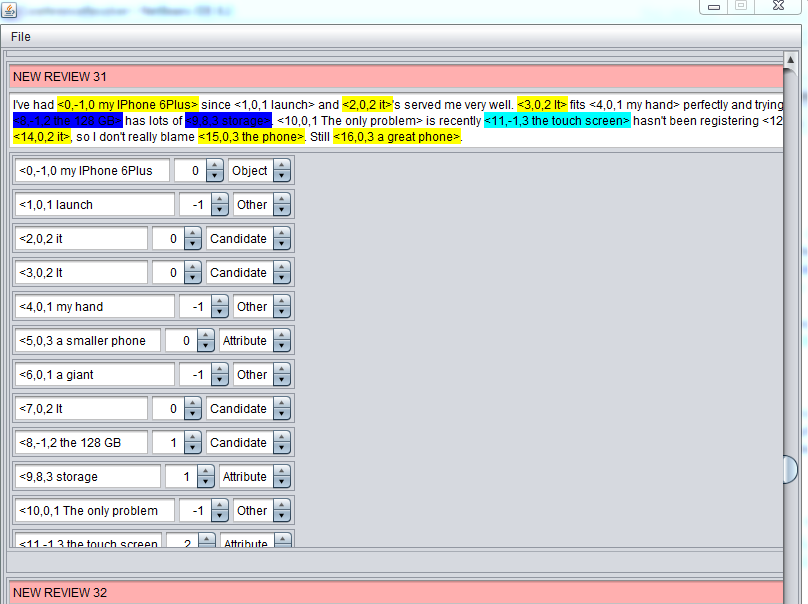
\includegraphics[scale=0.45]{images/markup_tool}				
			\caption{Công cụ gán nhãn dữ liệu đồng tham chiếu}				
		\end{figure}
	\end{frame}

	\subsection{Rút trích đặc trưng}
	\begin{frame}{Rút trích đặc trưng}				
		\begin{columns}[t]
			\begin{column}{0.7\textwidth}
			   	\begin{block}{Tạo các cặp cụm danh từ}
					Có ít nhất một đối tượng hoặc thuộc tính trong mỗi cặp cụm danh từ được tạo.
				\end{block}
				\begin{block}{Tạo các vectơ đặc trưng}										
					Tạo vectơ đặc trưng cho mỗi cặp cụm danh từ
				\end{block}
			\end{column}
			\begin{column}{0.3\textwidth}  %%<--- here
			 	\begin{figure}[H]
					\fontsize{13pt}{13}\selectfont
					\centering				
					\resizebox{20mm}{!}{\input{images/3.pdf_tex}}	
				\end{figure}
			\end{column}
		\end{columns}
		\begin{columns}[t]			
			\begin{column}{\textwidth}				
			   	\begin{figure}[H]
					\LARGE 
					\resizebox{100mm}{!}{\input{images/B3.pdf_tex}}										
				\end{figure}
			\end{column}			
		\end{columns}
	\end{frame}	

	\begin{frame}{Rút trích đặc trưng (tt)}		
		\begin{table}[]		
		\parbox{\textwidth}{
			\centering			
			\fontsize{8pt}{10}\selectfont		
			% Please add the following required packages to your document preamble:
% \usepackage{multirow}
% \usepackage[table,xcdraw]{xcolor}
% If you use beamer only pass "xcolor=table" option, i.e. \documentclass[xcolor=table]{beamer}
\begin{tabular}{|l|l|}
\hline
\textbf{Nhóm đặc trưng}                                                                                               & \textbf{Đặc trưng}                                               \\ \hline
{\color[HTML]{FE0000} }                                                                                               & {\color[HTML]{FE0000} Tính nhất quán về ý kiến}                  \\ \cline{2-2} 
\multirow{-2}{*}{{\color[HTML]{FE0000} \begin{tabular}[c]{@{}l@{}}Nhóm liên quan \\ Khai khoáng ý kiến\end{tabular}}} & {\color[HTML]{FE0000} Sự kết hợp giữa thực thể và từ chỉ ý kiến} \\ \hline
                                                                                                                      & NP1 là đại từ                                                    \\ \cline{2-2} 
                                                                                                                      & NP1 là đại từ quan hệ                                            \\ \cline{2-2} 
                                                                                                                      & NP2 là đại từ                                                    \\ \cline{2-2} 
                                                                                                                      & Tính thống nhất về số                                            \\ \cline{2-2} 
                                                                                                                      & Từ hạn định                                                      \\ \cline{2-2} 
                                                                                                                      & Từ chỉ trỏ                                                       \\ \cline{2-2} 
                                                                                                                      & Cả NP1 và NP2 đều là tên riêng                                   \\ \cline{2-2} 
                                                                                                                      & Giống nhau hoàn toàn                                             \\ \cline{2-2} 
                                                                                                                      & Danh từ chính giống nhau                                         \\ \cline{2-2} 
                                                                                                                      & Chuỗi con của nhau                                               \\ \cline{2-2} 
\multirow{-11}{*}{Nhóm cơ bản}                                                                                        & Khoảng cách                                                      \\ \hline
                                                                                                                      & Từ khóa "is" nằm ở giữa                                          \\ \cline{2-2} 
\multirow{-2}{*}{Khác}                                                                                                & Từ khóa "has" nằm ở giữa                                         \\ \hline
\end{tabular}	
			\caption{Các đặc trưng được sử dụng trong hệ thống \footnotemark \textsuperscript{,} \footnotemark}
		}
		\end{table}					
		\footnotetext[8]{Soon, Ng, and Lim. 2001.
	\textit{A machine learning approach to coreference resolution of noun phrases}.
	Computational Linguistics, 27(4):521–544.}
		\footnotetext[9]{Vincent Ng and Claire Cardie. 2002.
	\textit{Improving Machine Learning Approaches to Coreference Resolution}.
	Computational Linguistics, pages 104–111.}	
	\end{frame}	

	\begin{frame}{Rút trích đặc trưng (tt)}
		\begin{block}{Đặc trưng Sự kết hợp giữa thực thể và từ chỉ ý kiến (EOA)}			
			Từ chỉ ý kiến: good, bad, expensive, cheap,... \\ 
			Ví dụ:\\
			\textit{I love the \underline{nokia n95} but not sure how strong \underline{the flash} would be? And also \underline{it} is quite \underline{expensive}, so anyone got any ideas?} \\
			Hiện thực:
				\begin{itemize}
					\item{Xác định từ chỉ ý kiến kèm theo cụm danh từ.}
					\item{Xác định quan hệ từ chỉ ý kiến với các cụm danh từ. 
						\begin{equation*}
						PMI(NP,OW) = log\frac{(P(NP,OW)}{P(NP)\times P(OW)}
						\end{equation*}
				}
					\item{Xếp hạng các mối quan hệ giữa từ chỉ ý kiến với các cụm danh từ.}
				\end{itemize}

		\end{block}	
	\end{frame}

	\begin{frame}{Xây dựng dữ liệu học và kiểm tra (tt)}
		\begin{block}{Đặc trưng Tính nhất quán về ý kiến (SC)}		
			Ví dụ:\\
			\begin{itemize}				
				\item[$\bullet$]{\textit{\underline{The N73} is my favorite. \underline{It} can produce great pictures.}}
				\item[$\bullet$]{\textit{\underline{The K800} is awesome. \underline{That phone} has short battery life.}}
				\item[$\bullet$]{\textit{\underline{The XBR4} is brighter than \underline{the 5080}. Overall, \underline{it} is a great choice.}}
			\end{itemize}
			Hiện thực: \\
				\begin{itemize}
					\item{Xác định thiên hướng ý kiến (tích cực, tiêu cực) của mỗi cụm danh từ.}
					\item{So sánh thiên hướng giữa các cặp cụm danh từ.}
				\end{itemize}
			Giá trị đặc trưng: \\
			\begin{itemize}
				\item{SC = 0: Hai cụm danh từ nằm trong hai câu liên tiếp khác thiên hướng ý kiến}
				\item{SC = 1: Hai cụm danh từ nằm trong hai câu liên tiếp có cùng thiên hướng ý kiến}
				\item{SC = 2: Một trong hai cụm danh từ không xác định được thiên hướng ý kiến hoặc chúng không nằm trong hai câu liên tiếp}
			\end{itemize}									
		\end{block}	
				
	\end{frame}	

	\subsection{Phân loại và gom cụm}
	\begin{frame}{Phân loại và gom cụm}		
		\begin{columns}[t]
			\begin{column}{0.6\textwidth}
			   	\begin{block}{Phân loại}
					Giải thuật cây quyết định J48 (trên Weka) được sử dụng để phân loại cho các cặp ứng viên.
				\end{block}	
				\begin{block}{Tạo chuỗi đồng tham chiếu (Gom cụm)}
			   		(A,B) và (B,C) đồng tham chiếu $\Rightarrow$ Cụm đồng tham chiếu (A,B,C) (nhờ vào tính bắc cầu).
				\end{block}			
			\end{column}
			\begin{column}{0.4\textwidth}  %%<--- here
			 	\begin{figure}[H]
					\fontsize{13pt}{13}\selectfont
					\centering				
					\resizebox{20mm}{!}{\input{images/4.pdf_tex}}	
				\end{figure}
			\end{column}
		\end{columns}
		\begin{columns}[t]			
			\begin{column}{\textwidth}				
			   	\begin{figure}[H]
					\LARGE 
					\resizebox{100mm}{!}{\input{images/B4.pdf_tex}}										
				\end{figure}
			\end{column}			
		\end{columns}
	\end{frame}

	\section{Thực nghiệm và đánh giá}				
		\begin{frame}{Thực nghiệm và đánh giá}			
			\begin{block}{Dữ liệu thực nghiệm}
				\begin{itemize}
				 	\item Nguồn: \textit{amazon.com}, \textit{howardforums.com}
				 	\item Gồm 157 bài, mỗi bài trung bình 7-8 câu.
				 \end{itemize}				
			\end{block}
			\begin{figure}[H]
				\centering				
				\noindent\fbox{
				    \parbox{0.9\textwidth}{
				        The fact that the \textcolor{red}{GS5} is from Samsung makes it \textcolor{red}{the Z2}'s biggest competitor. \textcolor{red}{The Z2}'s strongest points are \textcolor{blue}{the side-mounted camera button}. \textcolor{red}{The Z2} has slightly louder \textcolor{blue}{speakers}, slightly better \textcolor{blue}{battery life} than \textcolor{red}{the GS5}. It has \textcolor{blue}{a fingerprint reader} for easier unlocking, a better looking \textcolor{blue}{screen} and a removable \textcolor{blue}{battery}. Between the two phones, I'd pick \textcolor{red}{the GS5} for its brighter \textcolor{blue}{display} and for the ease of use \textcolor{blue}{the fingerprint reader} brings. That said, watch out because \textcolor{red}{the GS5} doesn't use \textcolor{blue}{on-screen menu buttons} so handling it can be tricky unless you stick it in a \textcolor{blue}{case}.
			    	}
				}
				\caption{Ví dụ về một bài đánh giá (review) lấy từ amazon.com}				
			\end{figure}
		\end{frame}		

		\begin{frame}{Thực nghiệm và đánh giá (tt)}			
			\begin{block}{Phương pháp đánh giá}				
				\begin{itemize}
					\item{Kiểm chứng chéo (k-fold cross validation) với k=5}
					\item{Độ đo: Precision, Recall, F-measure}
					\item{Hệ đo: 
						\begin{itemize}
							\item[$\bullet$]{MUC} \footnotemark
							\item[$\bullet$]{B-CUBED} \footnotemark
							\item[$\bullet$]{CEAF-$\Phi_4$} \footnotemark
						\end{itemize}
					}					
				\end{itemize}		
			\end{block}					
			\footnotetext[10]{Vilain, Marc, John Burger, John Aberdeen, Dennis Connolly and Lynette Hirschman. 1995.
				\textit{A model-theoretic coreference scoring scheme}.
				In Proceedings of the 6th Message Understanding Conference (MUC-6), pages 45–52.}
			\footnotetext[11]{
				Amit Bagga and Breck Baldwin. 1998.
				\textit{Algorithms for Scoring Coreference Chains}.
				In The First International Conference on Language Resources and Evaluation Workshop on Linguistics Coreference.
			}
			\footnotetext[12]{
				Xiaoqiang Luo. 2005.
				\textit{On coreference resolution performance metrics}.
				In Proceedings of the Human Language Technology Conference and the 2005 Conference on Empirical Methods in Natural Language Processing, Vancouver, B.C., Canada, 6–8 October 2005, pages 25–32
			}
		\end{frame}		

		\begin{frame}{Thực nghiệm và đánh giá (tt)}			
			\begin{table}[]		
			\parbox{\textwidth}{
				\centering			
				\fontsize{8pt}{10}\selectfont		
				% Please add the following required packages to your document preamble:
% \usepackage{multirow}
% \usepackage[table,xcdraw]{xcolor}
% If you use beamer only pass "xcolor=table" option, i.e. \documentclass[xcolor=table]{beamer}
\begin{tabular}{|l|l|}
\hline
\textbf{Nhóm đặc trưng}                                                                       & \textbf{Đặc trưng/Nhóm đặc trưng}                                \\ \hline
                                                                                              & {\color[HTML]{FE0000} Tính nhất quán về ý kiến}                  \\ \cline{2-2} 
\multirow{-2}{*}{\begin{tabular}[c]{@{}l@{}}Nhóm liên quan\\ khai khoáng ý kiến\end{tabular}} & {\color[HTML]{3531FF} Sự kết hợp giữa thực thể và từ chỉ ý kiến} \\ \hline
                                                                                              & Nhóm cơ bản                                                      \\ \cline{2-2} 
\multirow{-2}{*}{Các nhóm cơ sở}                                                              & Khác                                                             \\ \hline
\end{tabular}	
				\caption{Tóm tắt các đặc trưng được sử dụng trong hệ thống}
			}
			\end{table}	
			\begin{block}{Các hệ thống được đánh giá}								
				\begin{itemize}
					\item{Hệ thống cơ sở: Nhóm liên quan ngữ pháp + Nhóm liên quan từ vựng + Nhóm thuộc tính khác.}
					\item{Hệ thống SC: Hệ thống cơ sở + \textit{Tính nhất quán về ý kiến (SC)}.}
					\item{Hệ thống EOA: Hệ thống cơ sở + \textit{Sự kết hợp giữa thực thể và từ chỉ ý kiến (EOA)}.}
					\item{Hệ thống đầy đủ: Tất cả đặc trưng.}
				\end{itemize}								
			\end{block}				
		\end{frame}

		\begin{frame}[t]{Thực nghiệm và đánh giá (tt)}								
			\begin{columns}[t]
				\begin{column}{\textwidth}
					\begin{figure}[H] 			
						\centering					
						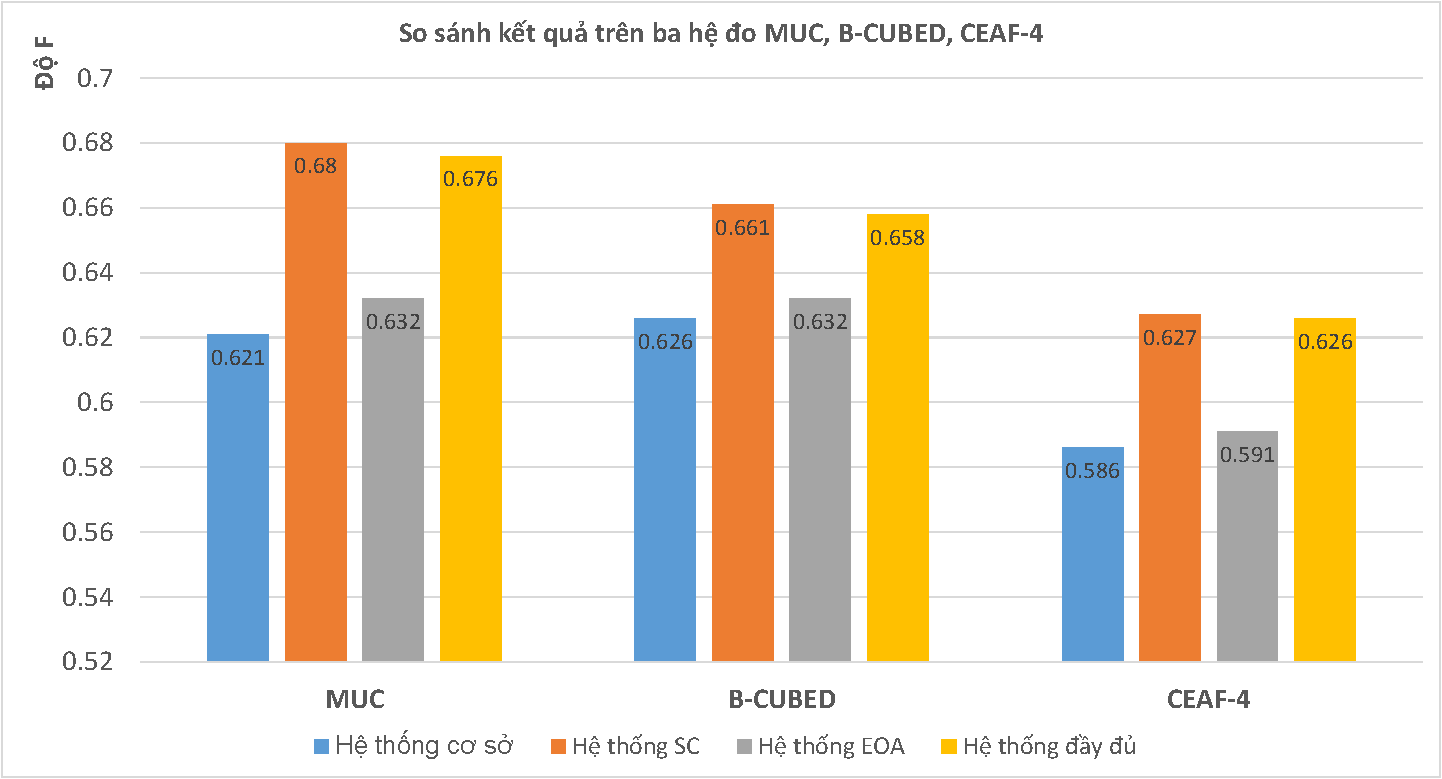
\includegraphics[scale=0.38]{charts/chart_comparison.pdf}									
					\end{figure} 				
				\end{column}
			\end{columns}
			\begin{columns}[t]
				\begin{column}{\textwidth}
					\begin{block}{Nhận xét}
						\footnotesize		
						\begin{itemize}
							\item{Đặc trưng liên quan đến Khai khoáng ý kiến đã ảnh hưởng tích cực đến kết quả}
							\item{Đặc trưng \textit{Tính nhất quán về ý kiến (SC)} đã có ảnh hưởng tương đối lớn đến hệ thống}
							\item{Đặc trưng \textit{Sự kết hợp giữa thực thể và từ chỉ ý kiến (EOA)} ít có ảnh hưởng tích cực đến hệ thống}
							\item{Việc kết hợp hai đặc trưng mới \textit{Tính nhất quán về ý kiến (SC)} và \textit{Sự kết hợp giữa thực thể và từ chỉ ý kiến (EOA)} vẫn còn gặp vấn đề}
						\end{itemize}			
					\end{block}
				\end{column}				
			\end{columns}						
		\end{frame}					

	\section{Tổng kết}
		\begin{frame}{Tổng kết}			
			\begin{block}{Kết quả đạt được}
				\begin{itemize}
					\item Từ những kiến thức về Phân giải đồng tham chiếu và Khai khoáng ý kiến, đưa ra được phương pháp giải quyết bài toán.
					\item Hiện thực hệ thống dựa trên phương pháp đề xuất, cho kết quả đầu ra khả quan.				
				\end{itemize}
			\end{block}
			\begin{block}{Khó khăn, hạn chế}
				\begin{itemize}
					\item Dữ liệu tự thu thập và tự gán nhãn, công đoạn gán nhãn có thể gặp một số sai sót. 
					\item Do giới hạn về thời gian nên chưa kịp thử nghiệm cho tiếng Việt.				
				\end{itemize}
			\end{block}
		\end{frame}
	
		\begin{frame}{Tổng kết (tt)}			
			\begin{block}{Hướng phát triển}
				\begin{itemize}
					\item Tìm thêm các đặc trưng mới liên quan đến Khai khoáng ý kiến để tăng hiệu suất hệ thống.
					\item Cải thiện đặc trưng \textit{Sự kết hợp giữa thực thể và từ chỉ ý kiến}.
					\item Thử nghiệm cho tiếng Việt.
				\end{itemize}
			\end{block}
		\end{frame}

		\begin{frame}{Hết phần trình bày}
			\Huge
			\centering
			\fontsize{35pt}{35}\selectfont
			\textit{Cảm ơn hội đồng đã lắng nghe!}			
		\end{frame}

	\section{Phụ lục}
		\begin{frame}{Phụ lục: Các hệ đo}
			\begin{block}{Hệ đo MUC}
				\begin{center}
					\inlineitem{\scalebox{1.5}{$P = \frac{\sum \left(|R_i| - |p \left(R_i\right)|\right)}{\sum_{|R_i| - 1}}$}}
					\inlineitem{\scalebox{1.5}{$R = \frac{\sum \left(|S_i| - |p \left(S_i\right)|\right)}{\sum_{|S_i| - 1}}$}}
				\end{center}
			\end{block}
			\begin{block}{Hệ đo CEAF-$\Phi_4$}
				\begin{center}						
					\inlineitem{\scalebox{1.5}{$P = \frac{\Phi \left(g*\right)}{\sum_{S_i \in S*}\Phi_4 \left(S_i, S_i\right)}$}}
					\inlineitem{\scalebox{1.5}{$R = \frac{\Phi \left(g*\right)}{\sum_{R_i \in R*}\Phi_4 \left(R_i, S_j\right)}$}}
				\end{center}
			\end{block}
		\end{frame}

		\begin{frame}{Phụ lục: Các hệ đo (tt)}
			\begin{block}{Hệ đo B-CUBED}
				\begin{center}
					\begin{itemize} 
					\item{\scalebox{1.5}{$P = \frac{1}{n} \sum_{i=1}^{n} \frac{\sum_{j=1}^{|p (S_i)|} |P_{ij}|*\left(|S_i| - |P_{ij}|\right)} {|S_{i}|^2}$}}
					\item{\scalebox{1.5}{$R = \frac{1}{m} \sum_{i=1}^{m} \frac{\sum_{j=1}^{|p (R_i)|} |P'_{ij}|*\left(|S_i| - |P'_{ij}|\right)} {|R_{i}|^2}$}}
					\end{itemize}
				\end{center}
			\end{block}	
			\begin{block}{Công thức tính F}
				\begin{center}									
					\scalebox{1.5}{$F = \frac{2PR}{P+R}$}
				\end{center}
			\end{block}					
		\end{frame}

		\begin{frame}{Phụ lục: Pointwise Mutual Information (PMI)}
			\footnotetext[13]{Fano, R., 1961.
				\textit{Transmission of Information}.
				MIT Press Cambridge, Massachussetts. 
			}
				\begin{center}
						\begin{equation*}
						PMI(NP,OW) = log\frac{(P(NP,OW)}{P(NP)\times P(OW)}
						\end{equation*}
				\end{center}
				\begin{itemize} 
					\item{P(NP): Xác suất cụm danh từ xuất hiện trong tập dữ liệu T.}
					\item{P(OW): Xác suất từ chỉ ý kiến xuất hiện trong tập dữ liệu T.}
					\item{P(NP,OW): Xác suất cụm danh từ và từ chỉ ý kiến cùng xuất hiện trong một câu trong tập dữ liệu T.} \footnotemark
				\end{itemize}
		\end{frame}

		\begin{frame}{Phụ lục: Công cụ CRFChunker}
			\begin{block}{Công cụ CRFChunker}
				\begin{itemize}
					\item{Độ F = 95.77\%}
					\item{Tốc độ gom cụm từ (chunking speed) = 700 câu/giây \footnotemark}
				\end{itemize}
			\end{block}
			\begin{figure}[H]
				\centering
				\footnotesize				
				\noindent\fbox{
				    \parbox{0.9\textwidth}{
				    	The/DT/B-NP Note/NN/I-NP 3/CD/I-NP is/VBZ/B-VP a/DT/B-NP lot/NN/I-NP lighter/JJR/B-ADVP than/IN/B-PP my/PRP\$/B-NP HTC/NNP/I-NP EVO/NNP/I-NP ././O
				    	\\
				    	\\
				        It/PRP/B-NP 's/VBZ/B-VP very/RB/B-ADJP fast/JJ/I-ADJP and/CC/O has/VBZ/B-VP so/RB/B-NP many/JJ/I-NP features/NNS/I-NP that/IN/B-SBAR an/DT/B-NP IPhone5/NN/I-NP ca/MD/B-VP n't/RB/I-VP touch/VB/I-VP ././O 
				        \\
				        \\
						I/PRP/B-NP love/VBP/B-VP the/DT/B-NP camera/NN/I-NP features/NNS/I-NP and/CC/O it/PRP/B-NP takes/VBZ/B-VP great/JJ/B-NP pictures/NNS/I-NP ././O
			    	}
				}
				\caption{Kết quả đầu ra của công cụ CRFChunker}				
			\end{figure}
			\footnotetext[14]{Xuan-Hieu Phan, \textit{CRFChunker: CRF English Phrase Chunker}, http://crfchunker.sourceforge.net/, 2006.}
		\end{frame}

		\begin{frame}{Phụ lục: Từ điển ý kiến và từ khóa so sánh}
			\begin{block}{Từ điển ý kiến}
				\begin{itemize}
					\item Dùng từ điển ý kiến (opinion lexicon) được cung cấp bởi Bing Liu \footnotemark
					\item Từ điển này gồm 6800 từ (tích cực + tiêu cực), được tập hợp bắt đầu từ bài báo (Hu và Liu, KDD-2004)
				\end{itemize}
			\end{block}
			\begin{block}{Từ khóa so sánh}
				Gồm có 3 nhóm:
				\begin{itemize}
					\item Từ có nhãn từ loại là JJR, RBR
					\item more/less + JJ/RB
					\item Các từ đặc biệt: beat, outperform,...
				\end{itemize}
			\end{block}
			\footnotetext[15]{http://www.cs.uic.edu/~liub/FBS/opinion-lexicon-English.rar}
		\end{frame}

		\begin{frame}{Công trình của Stoyanov và Cardie}
		\end{frame}

		\begin{frame}{Phụ lục: Công trình của Ding và Liu (2010)}
			\begin{figure}[H]
				\centering							
				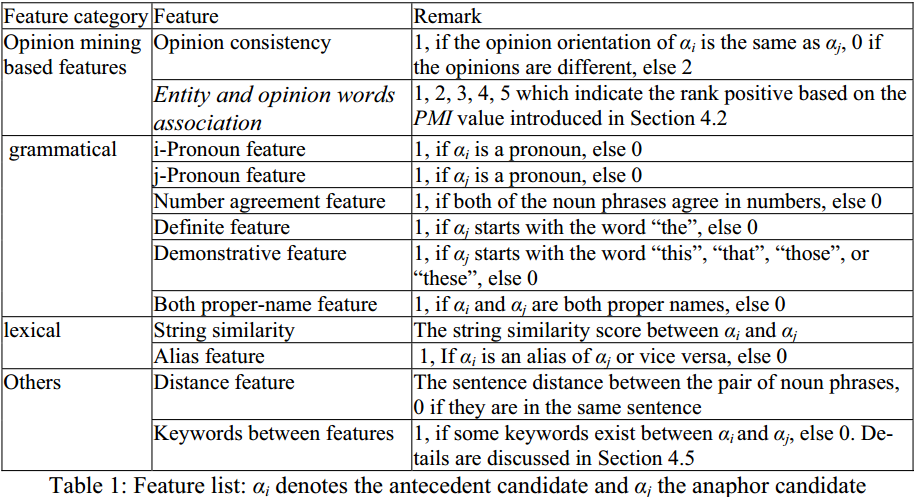
\includegraphics[scale=0.45]{images/base_features}				
				\caption{Các đặc trưng trích từ bài báo của Ding và Liu (2010)}				
			\end{figure}
		\end{frame}

		\begin{frame}{Phụ lục: Công trình của Ding và Liu (2010) (tt)}
			\begin{figure}[H]
				\centering							
				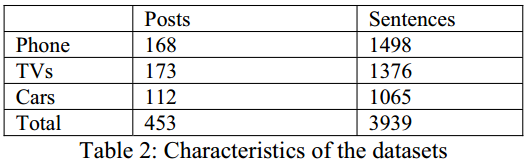
\includegraphics[scale=0.45]{images/base_result_1}				
				\caption{Thống kê về dữ liệu từ bài báo của Ding và Liu (2010)}				
			\end{figure}
			\begin{figure}[H]
				\centering							
				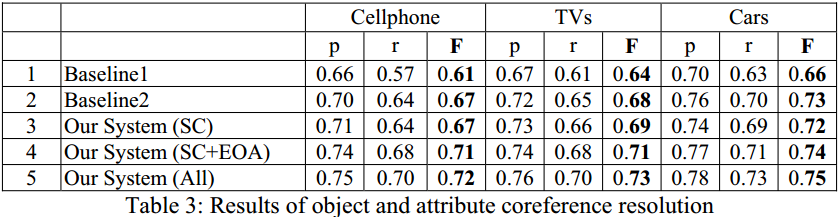
\includegraphics[scale=0.45]{images/base_result_2}				
				\caption{Các kết quả từ bài báo của Ding và Liu (2010)}				
			\end{figure}
		\end{frame}

		\begin{frame}{Phụ lục: Các công trình tìm đối tượng và thuộc tính}
			\begin{block}{Công trình của Hu và Liu (2004)}
				Bài toán \textit{Khai phá và tóm tắt các bài đánh giá (review) của người dùng}, với 3 công việc: 
				\begin{itemize}
					\item{Trích xuất các thuộc tính của đối tượng (mà họ gọi là \textit{feature}) được người dùng thể hiện ý kiến}
					\item{Đối với từng thuộc tính, xác định các câu thể hiện ý kiến kèm theo}
					\item{Tóm tắt kết quả}
				\end{itemize}
			\end{block}
			\begin{block}{Công trình của Popescu và Etzioni (2005)}
				Cải tiến công trình của Hu và Liu (2004) về phương pháp thực hiện và cho ra kết quả khả quan hơn
			\end{block}
		\end{frame}		

		\begin{frame}{Phụ lục: Mô hình cặp (mention pair)}
			\begin{figure}[H]
				\centering
				\scalebox{.8}{% Author: Rasmus Pank Roulund
% \documentclass{minimal}
% \usepackage{tikz}
% \usepackage[utf8]{vietnam}

% \begin{document}
% \usetikzlibrary{arrows,chains,positioning,scopes}

\tikzset{
    block/.style={draw,thick,text width=5em,minimum height=6.5em,minimum width=5em,align=center},
    arrow/.style={->, thick}
}
\begin{tikzpicture}
  {[start chain]
      \node[block,on chain] (N1) {Tập hợp các cụm danh từ};
      \node[block,on chain,join=by {arrow},right=1cm of N1] (N2) {Tạo tập các cặp cụm danh từ};
      \node[block,on chain,join=by {arrow},right=1cm of N2] (N3) {Phân loại các cặp cụm danh từ};
      \node[block,on chain,join=by {arrow},right=1cm of N3] (N4) {Kết hợp những cặp được phân loại đồng tham chiếu};
      \node[block,on chain,join=by {arrow},right=1cm of N4] (N5) {Các chuỗi đồng tham chiếu};
    }
      
  \end{tikzpicture}
% \end{document}}
				\caption{Ý tưởng các bước thực hiện trong Mô hình cặp}
				\label{fig:mentionpair}
			\end{figure}
		\end{frame}

		\begin{frame}{Phụ lục: Mô hình hướng thực thể (entity-mention)}
			\begin{figure}[H]
				\centering
				\scalebox{.8}{% Author: Rasmus Pank Roulund
% \documentclass{minimal}
% \usepackage{tikz}
% \usepackage[utf8]{vietnam}

% \begin{document}
% \usetikzlibrary{arrows,chains,positioning,scopes}

\tikzset{
    block/.style={draw,thick,text width=10em,minimum height=6.5em,minimum width=11em,align=center},
    arrow/.style={->, thick}
}
\begin{tikzpicture}
  {[start chain]
      \node[block,on chain] (N1) {Tập hợp các cụm danh từ};
      \node[block,on chain,join=by {arrow},right=1cm of N1] (N2) {Xem mỗi cụm danh từ là một chuỗi đồng tham chiếu};
      \node[block,on chain,join=by {arrow},right=1cm of N2] (N3) {Tạo các cặp chứa hai chuỗi đồng tham chiếu};
      \node[block,on chain,join=by {arrow},below=1cm of N3] (N4) {Phân loại các cặp đã tạo};
      \node[block,on chain,join=by {arrow},left=1cm of N4] (N5) {Nếu cặp nào được phân loại đồng tham chiếu, gộp hai chuỗi của cặp đó làm một};
      \node[block,on chain,join=by {arrow},left=1cm of N5] (N6) {Các chuỗi đồng tham chiếu};      
    }
      
  \end{tikzpicture}
% \end{document}}
				\caption{Một hiện thực điển hình của mô hình thực thể}
				\label{fig:entitymention}
			\end{figure}
		\end{frame}

		\begin{frame}{Phụ lục: Mô hình xếp hạng (ranking model)}
			\begin{figure}[H]
				\centering
				\scalebox{.8}{% Author: Rasmus Pank Roulund
% \documentclass{minimal}
% \usepackage{tikz}
% \usepackage[utf8]{vietnam}

% \begin{document}
% \usetikzlibrary{arrows,chains,positioning,scopes}

\tikzset{
    block/.style={draw,thick,text width=6em,minimum height=10em,minimum width=7em,align=center},
    arrow/.style={->, thick}
}
\begin{tikzpicture}
  {[start chain]
      \node[block,on chain] (N1) {Tập hợp các cụm danh từ};
      \node[block,on chain,join=by {arrow},right=1cm of N1] (N2) {Lọc lại các cụm danh từ có khả năng nằm trong chuỗi đồng tham chiếu};
      \node[block,on chain,join=by {arrow},right=1cm of N2] (N3) {Với một cụm danh từ, so sánh các ứng viên cụm danh từ nằm bên trái của nó};
      \node[block,on chain,join=by {arrow},right=1cm of N3] (N4) {Lựa chọn ứng viên có khả năng đồng tham chiếu cao nhất};
      \node[block,on chain,join=by {arrow},below=1cm of N4] (N5) {Tạo các cặp cụm danh từ đồng tham chiếu};
      \node[block,on chain,join=by {arrow},left=1cm of N5] (N6) {Kết hợp những cặp đồng tham chiếu};
      \node[block,on chain,join=by {arrow},left=1cm of N6] (N7) {Tạo các chuỗi đồng tham chiếu};      
    }
      
  \end{tikzpicture}
% \end{document}}
				\caption{Ý tưởng các bước của mô hình xếp hạng}
				\label{fig:rankingmodel}
			\end{figure}
		\end{frame}

		\begin{frame}{Phụ lục: Các đặc trưng được sử dụng}		
			\begin{table}[]		
			\parbox{\textwidth}{
				\centering			
				\fontsize{6pt}{7}\selectfont		
				\begin{tabular}{|l|l|l|}
\hline
Nhóm thuộc tính                                                                               & Thuộc tính                                                                           & Giải thích                                                                                                                                                                                                                                   \\ \hline
\multirow{2}{*}{\begin{tabular}[c]{@{}l@{}}Nhóm liên quan \\ khai khoáng ý kiến\end{tabular}} & Tính nhất quán về ý kiến                                                             & \begin{tabular}[c]{@{}l@{}}Bằng 1 nếu NP1 và NP2 có\\ cùng thiên hướng ý kiến. \\ Bằng 0 nếu chúng khác về \\ thiên hướng ý kiến. \\ Nếu không xác định được \\ thiên hướngý kiến cho NP1 \\ hoặc NP2 thì bằng 2.\end{tabular} \\ \cline{2-3} 
                                                                                              & \begin{tabular}[c]{@{}l@{}}Sự kết hợp giữa thực thể \\ và từ chỉ ý kiến\end{tabular} & \begin{tabular}[c]{@{}l@{}}Bằng 0,1,2,3,4,10 tùy vào \\ xếp hạng PMI\end{tabular}                                                                                                                                                            \\ \hline
\multirow{6}{*}{\begin{tabular}[c]{@{}l@{}}Nhóm liên quan \\ ngữ pháp\end{tabular}}           & NP1 là đại từ                                                                    & \begin{tabular}[c]{@{}l@{}}Bằng 1 nếu NP1 là đại từ, \\ ngược lại bằng 0\end{tabular}                                                                                                                                                    \\ \cline{2-3} 
                                                                                              & NP2 là đại từ                                                                     & \begin{tabular}[c]{@{}l@{}}Bằng 1 nếu NP2 là đại từ, \\ ngược lại bằng 0\end{tabular}                                                                                                                                                     \\ \cline{2-3} 
                                                                                              & Tính thống nhất về số                                                                & \begin{tabular}[c]{@{}l@{}}Bằng 1 nếu NP1 và NP2 \\ thống nhất về số (trong ngữ pháp),\\  ngược lại bằng 0\end{tabular}                                                                                                               \\ \cline{2-3} 
                                                                                              & Từ hạn định                                                                          & \begin{tabular}[c]{@{}l@{}}Bằng 1 nếu NP2 bắt đầu bằng \\ "the", ngược lại bằng 0\end{tabular}                                                                                                                                            \\ \cline{2-3} 
                                                                                              & Từ chỉ trỏ                                                                           & \begin{tabular}[c]{@{}l@{}}Bằng 1 nếu NP2 bắt đầu bằng \\ "this", "that", "these", those", \\ ngược lại bằng 0\end{tabular}                                                                                                               \\ \cline{2-3} 
                                                                                              & \begin{tabular}[c]{@{}l@{}}Cả NP1 và NP2 \\ đều là tên riêng\end{tabular} & \begin{tabular}[c]{@{}l@{}}Bằng 1 nếu NP1 và NP2 \\ đều là tên riêng, ngược lại \\ bằng 0\end{tabular}                                                                                                                            \\ \hline
\begin{tabular}[c]{@{}l@{}}Nhóm liên quan \\ từ vựng\end{tabular}                             & Tương tự về từ vựng                                                                  & \begin{tabular}[c]{@{}l@{}}Tính tương tự về mặt từ vựng \\ (trùng hoặc gần giống nhau)\end{tabular}                                                                                                                                          \\ \hline
\multirow{3}{*}{Khác}                                                                         & Khoảng cách                                                                          & \begin{tabular}[c]{@{}l@{}}Khoảng cách về câu chứa NP1 \\ và NP2. Nếu chúng nằm cùng \\ một câu thì bằng 0\end{tabular}                                                                                                               \\ \cline{2-3} 
                                                                                              & Từ khóa "is" nằm ở giữa                                                              & \begin{tabular}[c]{@{}l@{}}Bằng 1 nếu có "is" không đi kèm \\ với chỉ định so sánh nào nằm ở \\ giữa NP1 và NP2, ngược lại \\ thì bằng 0\end{tabular}                                                                                 \\ \cline{2-3} 
                                                                                              & Từ khóa "has" nằm ở giữa                                                             & \begin{tabular}[c]{@{}l@{}}Bằng 1 nếu có "has" nằm ở giữa \\ NP1 và NP2, ngược lại thì \\ bằng 0\end{tabular}                                                                                                                         \\ \hline
\end{tabular}	
				\caption{Các đặc trưng được sử dụng trong hệ thống}
			}
			\end{table}
		\end{frame}	

		\begin{frame}{Phụ lục: Các đặc trưng được sử dụng (tt)}				
			\begin{table}[]		
			\parbox{\textwidth}{
				\centering
				\fontsize{6pt}{7}\selectfont			
				\begin{tabular}{|l|l|l|}
\hline
Nhóm đặc trưng                                                                                & Đặc trưng                                                                            & Giải thích                                                                                                                                                                                                                      \\ \hline
\multirow{3}{*}{\begin{tabular}[c]{@{}l@{}}Nhóm liên quan\\ từ vựng\end{tabular}}             & Giống nhau hoàn toàn                                                                 & \begin{tabular}[c]{@{}l@{}}Bằng 1 nếu NP1 và NP2\\ giống nhau hoàn toàn về mặt\\ từ vựng\end{tabular}                                                                                                                           \\ \cline{2-3} 
                                                                                              & Danh từ chính giống nhau                                                             & \begin{tabular}[c]{@{}l@{}}Bằng true nếu NP1 và NP2 có\\ danh từ chính giống nhau,\\ ngược lại bằng false\end{tabular}                                                                                                                 \\ \cline{2-3} 
                                                                                              & Chuỗi con của nhau                                                                   & \begin{tabular}[c]{@{}l@{}}Bằng true nếu NP1 và NP2 là chuỗi\\ con (cha) của nhau, ngược lại\\ bằng false\end{tabular}                                                                                                                 \\ \hline
\multirow{3}{*}{Khác}                                                                         & Khoảng cách                                                                          & \begin{tabular}[c]{@{}l@{}}Khoảng cách về câu chứa NP1 \\ và NP2. Nếu chúng nằm cùng \\ một câu thì bằng 0\end{tabular}                                                                                                         \\ \cline{2-3} 
                                                                                              & Từ khóa "is" nằm ở giữa                                                              & \begin{tabular}[c]{@{}l@{}}Bằng true nếu có "is" không đi kèm \\ với chỉ định so sánh nào nằm ở \\ giữa NP1 và NP2, ngược lại \\ thì bằng false\end{tabular}                                                                           \\ \cline{2-3} 
                                                                                              & Từ khóa "has" nằm ở giữa                                                             & \begin{tabular}[c]{@{}l@{}}Bằng true nếu có "has" nằm ở giữa \\ NP1 và NP2, ngược lại thì \\ bằng false\end{tabular}                                                                                                                   \\ \hline
\end{tabular}	
				\caption{Các đặc trưng được sử dụng trong hệ thống (tt)}
			}
			\end{table}		
		\end{frame}

		\begin{frame}{Phụ lục: Kết quả thực nghiệm}
			\begin{table}[]
				\LARGE
				\centering
				\resizebox{\textwidth}{!}{								
				\begin{tabular}{|l|cx{1cm}c|cx{1cm}c|cx{1cm}c|c|c|c|c|c|c|}
				\hline
				                & \multicolumn{3}{c|}{Hệ đo MUC} & \multicolumn{3}{c|}{Hệ đo B3} & \multicolumn{3}{c|}{Hệ đo CEAF-$\Phi_4$} \\ \hline
				                & P        & R        & F        & P        & R        & F       & P         & R         & F         \\  \hline
				Hệ thống cơ sở  &  0.757        &  0.534       &  0.621       &   0.794       &   0.524       & 0.626        & 0.621          & 0.557          &   0.586  \\ \hline
				Hệ thống SC     &   0.742       &  0.630        &  0.680        & 0.735         &  0.608        &  0.661       &  0.666         & 0.593          & 0.627          \\ \hline
				Hệ thống EOA 	&   0.735       &  0.558        &  0.632        & 0.766         &  0.542        &  0.632       &  0.616         & 0.568          & 0.591          \\ \hline
				Hệ thống đầy đủ &  0.730        &   0.632       &  0.676        & 0.724         &  0.610        &   0.658      &  0.661         &  0.594         &  0.626         \\ \hline
				\end{tabular}
				}
				\caption{Kết quả thực nghiệm}
			\end{table}	
		\end{frame}

		\begin{frame}{Phụ lục: Phân tích}			
			\begin{itemize}
				\item{Số lượng từ chỉ ý kiến trong tập dữ liệu vẫn chưa nhiều (chỉ có 442 trong số 2634 cụm từ chỉ đối tượng, thuộc tính có từ chỉ ý kiến đi kèm) $\Rightarrow$ Đặc trưng EOA vẫn chưa ảnh hưởng nhiều đến hệ thống.}
				\item{Các từ chỉ ý kiến trong tập dữ liệu vẫn chưa có tính đặc trưng cao, ví dụ như tính từ \textit{good}, \textit{nice}, \textit{better}, \textit{great}.}									
				\item{Giải thuật tìm thiên hướng ý kiến gắn với đối tượng/thuộc tính được nêu ra trong câu vẫn còn đơn giản và chỉ cho kết quả đúng đối với các câu tương đối đơn giản.}
			\end{itemize}			
		\end{frame}

		\begin{frame}{Phụ lục: Phân tích (tt)}			
			\begin{itemize}
				\item{Mỗi bài đánh giá xuất hiện nhiều đối tượng và thuộc tính $\Rightarrow$ Khó xác định đồng tham chiếu nếu không dựa vào hai đặc trưng liên quan đến khai khoáng ý kiến.}
				\item{Một số trường hợp một đối tượng được diễn tả bởi nhiều tên gọi khác nhau mà không đặc trưng nào trong hệ thống phát hiện ra được. Ví dụ: \textit{the GS3}, \textit{the Samsung S3}, \textit{a new S3 SGH-I747 (US model) ATT phone}.}
				\item{Đặc trưng \textit{Danh từ chính giống nhau} ảnh hưởng nhiều đến độ đúng đắn của hệ thống nhưng có một số trường hợp bắt sai. Ví dụ: \textit{the camera quality} và \textit{the image quality}.}
			\end{itemize}			
		\end{frame}

\end{document}